\documentclass{article}
\documentclass[a4paper,12pt]{article}
\usepackage[english]{babel}
\usepackage[utf8]{inputenc}
\usepackage{amsfonts}
\usepackage{indentfirst}
\usepackage[T1]{fontenc}
\usepackage{amsmath}
\usepackage{hyperref}
\usepackage{graphicx}
\usepackage{subfig}
\usepackage[export]{adjustbox}

\textwidth\paperwidth
\advance\textwidth -45mm
\oddsidemargin 18mm
\advance\oddsidemargin -18mm
\evensidemargin 18mm
\advance\evensidemargin -18mm
\topmargin -30mm
\advance\topmargin 17mm
\setlength\textheight{45\baselineskip}
\addtolength\textheight{\topskip}
\marginparwidth 15mm


\title{
\textbf{Human Recognition by Biometric Methods}\\
\bigskip
\textbf{Face detection and classification}\\
\bigskip
}
\author{Mikołaj Małkiński}
\date{7 June 2018}

\begin{document}

    \maketitle

    \section{Introduction}\label{sec:introduction}

    The goal of this task was to design, implement and train YOLO object detection system (YOLOv3 was chosen) for detecting faces of Polish rappers.
    Then, the extracted face should be piped to previously trained model in order to classify it.

    The original dataset defined around 700 hundred bounding boxes for faces.
    Several boxes could refer to the same image.
    The dataset was split automatically into two parts by Keras, using 80\% of the data for training and remaining 20\% for validation.

    The models are resizing the images before processing, so data of arbitrary size can be used.
    However, it is important to note that images have to be in the same format (\textit{jpg} used in this case).
    Therefore, part of the pre-processing involves converting images from \textit{png} format to \textit{jpg}.
    Lack of this conversion caused unbearable accuracy - close to 0\%.

    The project consists of following scripts:
    \begin{itemize}
        \item \textit{detect\_classify} - detects faces in image and predicts their classes,
        \item \textit{evaluate} - evaluates model accuracy (Mean Average Precision at 0.5) and loss using specified configuration file,
        \item \textit{reproduce\_results} - creates plots shown in the report,
        \item \textit{train} - trains detection system using specified configuration file.
    \end{itemize}

    \newpage

    \section{Analysis of results}\label{sec:analysisOfResults}

    Figure~\ref{fig:compare1} presents comparison of results using two configurations, which differences are described in the Figure~\ref{fig:configurations1}.
    Min and max input size define the range to vary the size of the image during training (should be a multiple of 32).
    It can be observed that although bigger input sizes resulted in faster mAP improvement, the final mAP@0.5 after 24 epochs rounded to 2 digits after the comma, was the same - $91\%$.

    \begin{figure}[!h]
        \centering
        \begin{tabular}{cccc}
            \textbf{Configuration} & \textbf{Min input size} & \textbf{Max input size} & \textbf{Batch size} \\
            1 & 128 & 288 & 4 \\
            2 & 288 & 448 & 2
        \end{tabular}
        \caption{Details of configurations}
        \label{fig:configurations1}
    \end{figure}

    \begin{figure}[!h]
        \centering
        \begin{tabular}{cc}
            \subfloat[Loss]{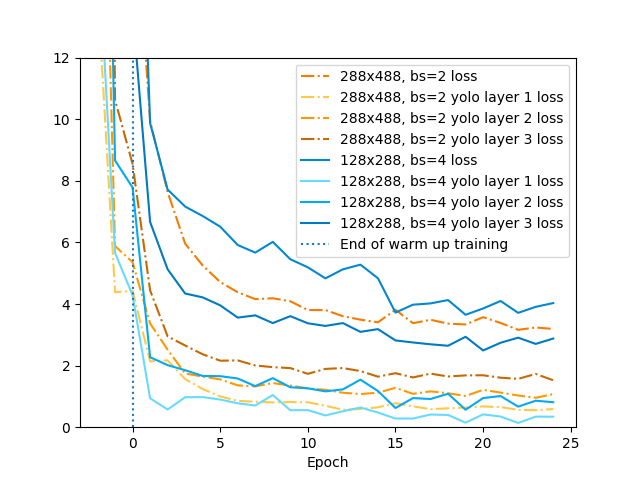
\includegraphics[width = 0.5\textwidth]{plots/compare_loss_face_01_06_15-25-face_05_06_15-08.png}} &
            \subfloat[Mean Average Precision at 0.5]{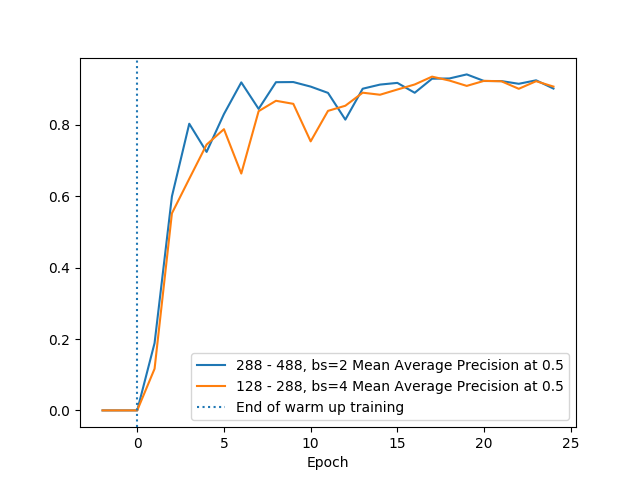
\includegraphics[width = 0.5\textwidth]{plots/compare_map_face_01_06_15-25-face_05_06_15-08.png}} \\
        \end{tabular}
        \caption{Comparison of two configurations}
        \label{fig:compare1}
    \end{figure}

\end{document}
